% Options for packages loaded elsewhere
\PassOptionsToPackage{unicode}{hyperref}
\PassOptionsToPackage{hyphens}{url}
%
\documentclass[
  12pt,
]{article}
\usepackage{lmodern}
\usepackage{amsmath}
\usepackage{ifxetex,ifluatex}
\ifnum 0\ifxetex 1\fi\ifluatex 1\fi=0 % if pdftex
  \usepackage[T1]{fontenc}
  \usepackage[utf8]{inputenc}
  \usepackage{textcomp} % provide euro and other symbols
  \usepackage{amssymb}
\else % if luatex or xetex
  \usepackage{unicode-math}
  \defaultfontfeatures{Scale=MatchLowercase}
  \defaultfontfeatures[\rmfamily]{Ligatures=TeX,Scale=1}
  \setmainfont[]{Times New Roman}
\fi
% Use upquote if available, for straight quotes in verbatim environments
\IfFileExists{upquote.sty}{\usepackage{upquote}}{}
\IfFileExists{microtype.sty}{% use microtype if available
  \usepackage[]{microtype}
  \UseMicrotypeSet[protrusion]{basicmath} % disable protrusion for tt fonts
}{}
\makeatletter
\@ifundefined{KOMAClassName}{% if non-KOMA class
  \IfFileExists{parskip.sty}{%
    \usepackage{parskip}
  }{% else
    \setlength{\parindent}{0pt}
    \setlength{\parskip}{6pt plus 2pt minus 1pt}}
}{% if KOMA class
  \KOMAoptions{parskip=half}}
\makeatother
\usepackage{xcolor}
\IfFileExists{xurl.sty}{\usepackage{xurl}}{} % add URL line breaks if available
\IfFileExists{bookmark.sty}{\usepackage{bookmark}}{\usepackage{hyperref}}
\hypersetup{
  pdftitle={Methane Emissions Status for Manure Management Across the USA},
  pdfauthor={Nadia Swit and Kendra Sultzer},
  hidelinks,
  pdfcreator={LaTeX via pandoc}}
\urlstyle{same} % disable monospaced font for URLs
\usepackage[margin=2.54cm]{geometry}
\usepackage{longtable,booktabs}
\usepackage{calc} % for calculating minipage widths
% Correct order of tables after \paragraph or \subparagraph
\usepackage{etoolbox}
\makeatletter
\patchcmd\longtable{\par}{\if@noskipsec\mbox{}\fi\par}{}{}
\makeatother
% Allow footnotes in longtable head/foot
\IfFileExists{footnotehyper.sty}{\usepackage{footnotehyper}}{\usepackage{footnote}}
\makesavenoteenv{longtable}
\usepackage{graphicx}
\makeatletter
\def\maxwidth{\ifdim\Gin@nat@width>\linewidth\linewidth\else\Gin@nat@width\fi}
\def\maxheight{\ifdim\Gin@nat@height>\textheight\textheight\else\Gin@nat@height\fi}
\makeatother
% Scale images if necessary, so that they will not overflow the page
% margins by default, and it is still possible to overwrite the defaults
% using explicit options in \includegraphics[width, height, ...]{}
\setkeys{Gin}{width=\maxwidth,height=\maxheight,keepaspectratio}
% Set default figure placement to htbp
\makeatletter
\def\fps@figure{htbp}
\makeatother
\setlength{\emergencystretch}{3em} % prevent overfull lines
\providecommand{\tightlist}{%
  \setlength{\itemsep}{0pt}\setlength{\parskip}{0pt}}
\setcounter{secnumdepth}{5}
\ifluatex
  \usepackage{selnolig}  % disable illegal ligatures
\fi

\title{Methane Emissions Status for Manure Management Across the USA}
\usepackage{etoolbox}
\makeatletter
\providecommand{\subtitle}[1]{% add subtitle to \maketitle
  \apptocmd{\@title}{\par {\large #1 \par}}{}{}
}
\makeatother
\subtitle{\url{https://github.com/sultzerk/SultzerSwit_ENV872_EDA_FinalProject.git}}
\author{Nadia Swit and Kendra Sultzer}
\date{}

\begin{document}
\maketitle

\newpage
\tableofcontents 
\newpage

\textbf{List of Tables}

\begin{enumerate}
\def\labelenumi{\arabic{enumi}.}
\tightlist
\item
  Table 1: Structure of Variables of Interest in
  Analysis\ldots\ldots\ldots\ldots\ldots\ldots\ldots\ldots\ldots.6
  \newpage

  \listoffigures 
  \newpage
\end{enumerate}

\hypertarget{rationale-and-research-questions}{%
\section{Rationale and Research
Questions}\label{rationale-and-research-questions}}

For this project, the area of interest was manure management and
greenhouse gas emissions created by livestock. The initial dataset
considered methane, nitrous oxide, and carbon dioxide. Research revealed
that ``livestock are reckoned to be responsible for up to 14\% of all
greenhouse emissions from human activities'' (Watts, 2019). Considering
the magnitude of industrial agriculture, we wanted to see how livestock
factored into emissions. When examining different emission types, this
study focused on methane because it is a very detrimental greenhouse
gas, trapping heat at a rate 25 times greater than carbon dioxide
(Watts, 2019). Pertaining to this study, methane gas is produced by the
anaerobic decomposition of manure stored or treated. Research and data
availability led to these two research questions:

\begin{itemize}
\item
  Question 1: Have methane emissions changed over time?
\item
  Question 2: Does the average methane emission rate differ between
  livestock?
\end{itemize}

\newpage

\hypertarget{dataset-information}{%
\section{Dataset Information}\label{dataset-information}}

The dataset used for this project was retrieved from the Food \&
Agriculture Organization of the United Nations (FAO), specifically from
FAOSTAT. FAOSTAT provides free access to statistics pertaining to
agriculture for over 245 countries. This analysis focused on emissions
in the United States. Emissions were computed following the 2006
Guidelines for National GHG Inventories of the Intergovernmental Panel
on Climate Change (IPCC). Methane emissions were estimated at the
country level by multiplying the number of livestock in heads by the
IPCC emission factors (FAO, 2020).

\hypertarget{data-wrangling-steps}{%
\subsection{Data Wrangling Steps}\label{data-wrangling-steps}}

The first step of data wrangling was viewing a summary of the full raw
data to determine how to best filter it for our research question needs.

Next, to make the dataset more manageable, specific columns to retain
were filtered. The main variable of interest, methane emissions, was
included, and we only focused on historical data.

In order to effectively conduct a time series analysis, we grouped by
years and summarized the mean methane emissions for all livestock.

Next, the pivot\_wider function was used to separate the livestock from
the same column into separate variables with their associated methane
emission values. This allowed separate time series to be run on the
desired livestock.

\hypertarget{data-structure}{%
\subsection{Data Structure}\label{data-structure}}

\textbf{Table 1: Structure of Variables of Interest in Analysis}

\begin{longtable}[]{@{}llll@{}}
\toprule
\begin{minipage}[b]{(\columnwidth - 3\tabcolsep) * \real{0.21}}\raggedright
\textbf{Variables}\strut
\end{minipage} &
\begin{minipage}[b]{(\columnwidth - 3\tabcolsep) * \real{0.32}}\raggedright
\textbf{Units}\strut
\end{minipage} &
\begin{minipage}[b]{(\columnwidth - 3\tabcolsep) * \real{0.26}}\raggedright
\textbf{Ranges}\strut
\end{minipage} &
\begin{minipage}[b]{(\columnwidth - 3\tabcolsep) * \real{0.20}}\raggedright
\textbf{Central Tendencies}\strut
\end{minipage}\tabularnewline
\midrule
\endhead
\begin{minipage}[t]{(\columnwidth - 3\tabcolsep) * \real{0.21}}\raggedright
Total Methane Emissions\strut
\end{minipage} &
\begin{minipage}[t]{(\columnwidth - 3\tabcolsep) * \real{0.32}}\raggedright
gigagrams (gg) CH4\strut
\end{minipage} &
\begin{minipage}[t]{(\columnwidth - 3\tabcolsep) * \real{0.26}}\raggedright
0-670.9518\strut
\end{minipage} &
\begin{minipage}[t]{(\columnwidth - 3\tabcolsep) * \real{0.20}}\raggedright
102.2441\strut
\end{minipage}\tabularnewline
\begin{minipage}[t]{(\columnwidth - 3\tabcolsep) * \real{0.21}}\raggedright
Item\strut
\end{minipage} &
\begin{minipage}[t]{(\columnwidth - 3\tabcolsep) * \real{0.32}}\raggedright
Animal\strut
\end{minipage} &
\begin{minipage}[t]{(\columnwidth - 3\tabcolsep) * \real{0.26}}\raggedright
13 animals: asses, cattle, chicken, ducks, goats, horses, mules, sheep,
swine, turkey\strut
\end{minipage} &
\begin{minipage}[t]{(\columnwidth - 3\tabcolsep) * \real{0.20}}\raggedright
\strut
\end{minipage}\tabularnewline
\begin{minipage}[t]{(\columnwidth - 3\tabcolsep) * \real{0.21}}\raggedright
Time\strut
\end{minipage} &
\begin{minipage}[t]{(\columnwidth - 3\tabcolsep) * \real{0.32}}\raggedright
years\strut
\end{minipage} &
\begin{minipage}[t]{(\columnwidth - 3\tabcolsep) * \real{0.26}}\raggedright
1980-2018 (predicted 2030 and 2050)\strut
\end{minipage} &
\begin{minipage}[t]{(\columnwidth - 3\tabcolsep) * \real{0.20}}\raggedright
\strut
\end{minipage}\tabularnewline
\bottomrule
\end{longtable}

\newpage

\hypertarget{exploratory-analysis}{%
\section{Exploratory Analysis}\label{exploratory-analysis}}

When considering our first research question, it is apparent there is a
general increasing trend over time (Figure 1). Analysis focused on
investigating whether this trend was significant. There is a sharp
decrease in methane emissions at the beginning of the dataset
(\textasciitilde1980-1985) that might warrant investigation later.

\begin{figure}
\centering
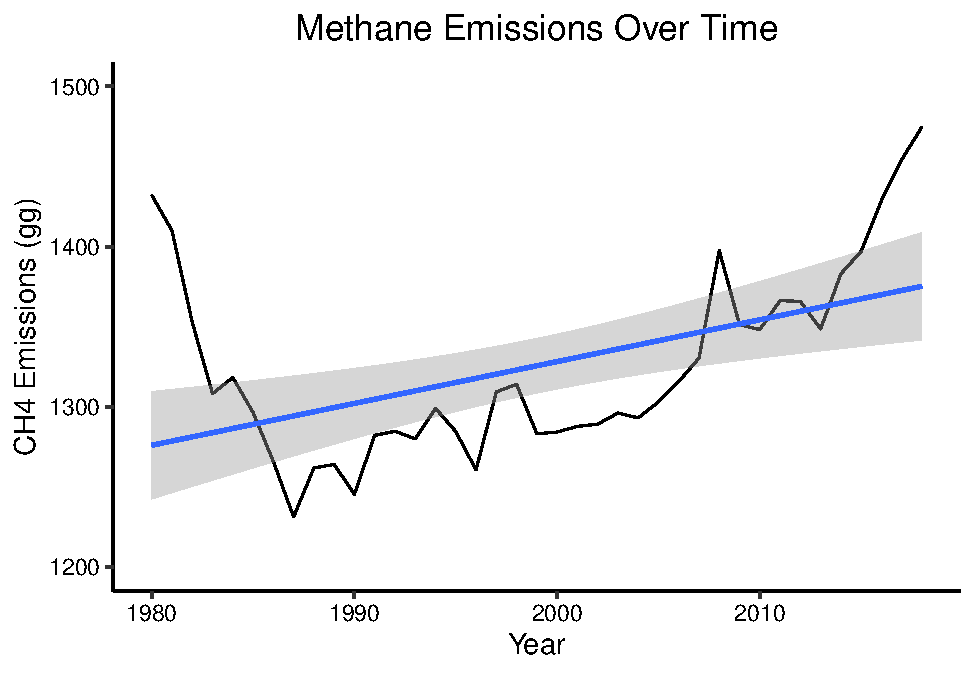
\includegraphics{SultzerSwit_ENV872_Project_files/figure-latex/unnamed-chunk-2-1.pdf}
\caption{Methane Emissions Over Time}
\end{figure}

We also visualized total methane emissions for each animal from
1980-2018 (Figure 2). It is evident that dairy cattle and market swine
had the highest emission rates. Analysis focused on investigating
whether these two livestock had significant emission trends.

\begin{figure}
\centering
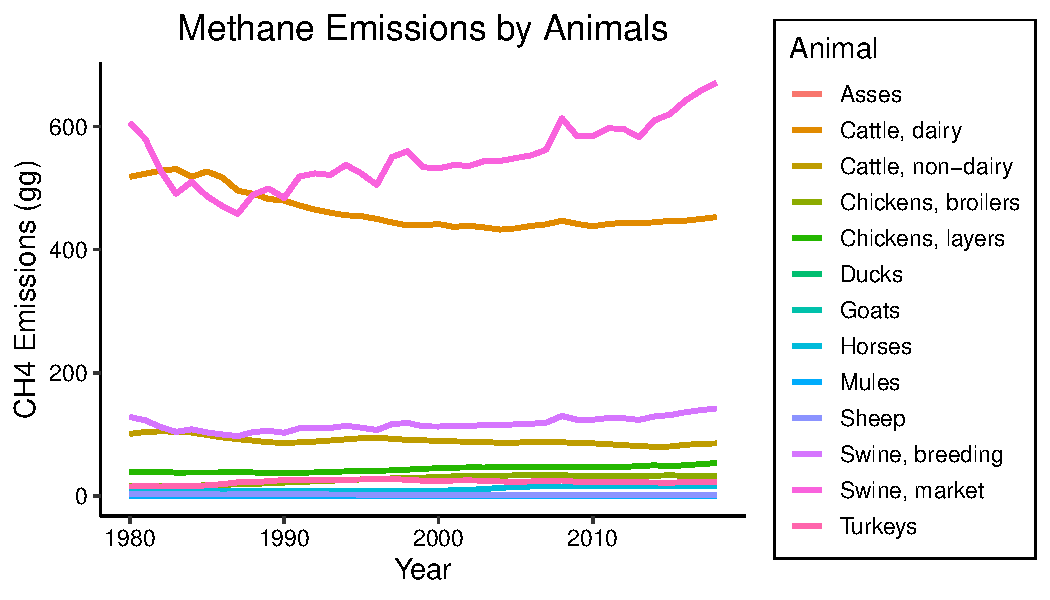
\includegraphics{SultzerSwit_ENV872_Project_files/figure-latex/unnamed-chunk-3-1.pdf}
\caption{Methane Emissions by Animals}
\end{figure}

Our second research question focused on the different emission rates
between animals. When exploring a boxplot showing the different rates
(Figure 3), it is suspected that there might be statistical differences.
For example, dairy cattle and market swine had much higher rates than
others. Analysis focused on investigating which rates were statistically
different from others.

\begin{figure}
\centering
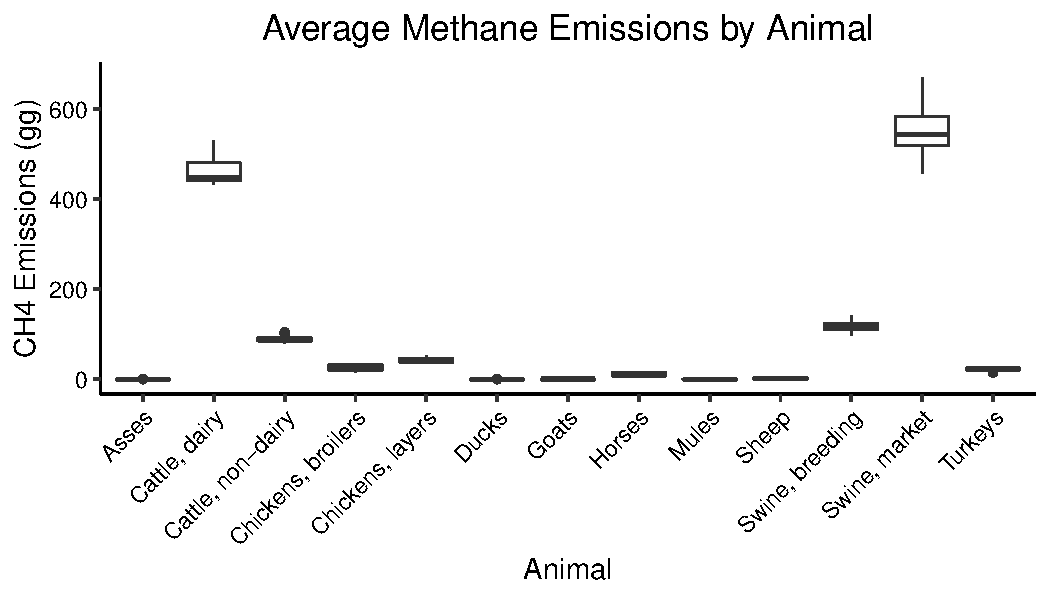
\includegraphics{SultzerSwit_ENV872_Project_files/figure-latex/viewing boxplot of methane by animal-1.pdf}
\caption{Average Methane Emissions by Animal}
\end{figure}

Additionally, to understand how the number of animals can influence
total methane emissions, we visualized how head of animals differed
between livestock category. Total livestock was visualized in Figure 4.
To control for the the higher proportion of chickens, we removed them
from the plot in Figure 5.

\begin{figure}
\centering
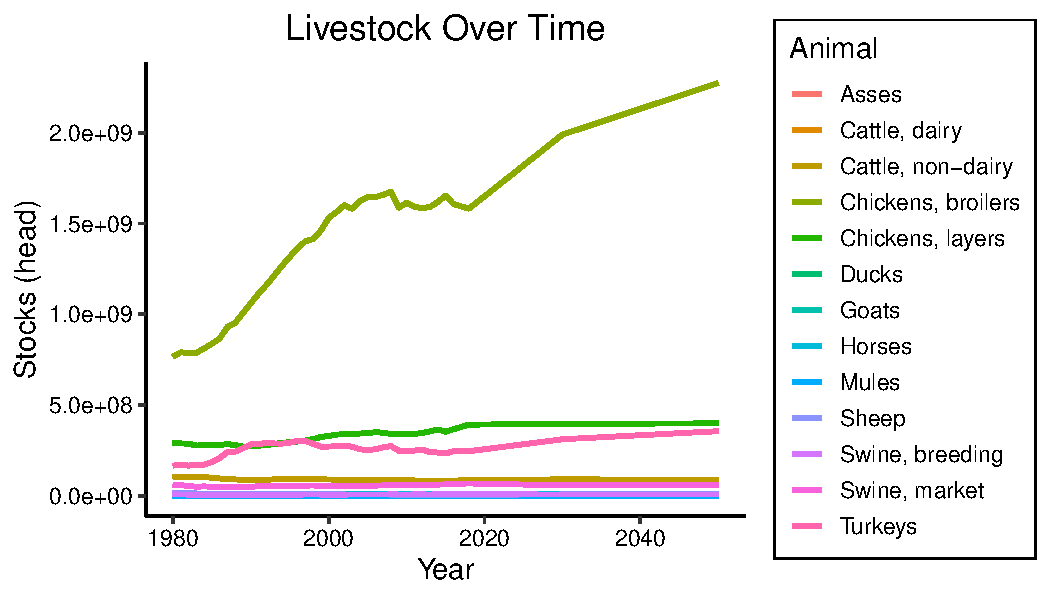
\includegraphics{SultzerSwit_ENV872_Project_files/figure-latex/animal.head-1.pdf}
\caption{Livestock Over Time}
\end{figure}

\begin{figure}
\centering
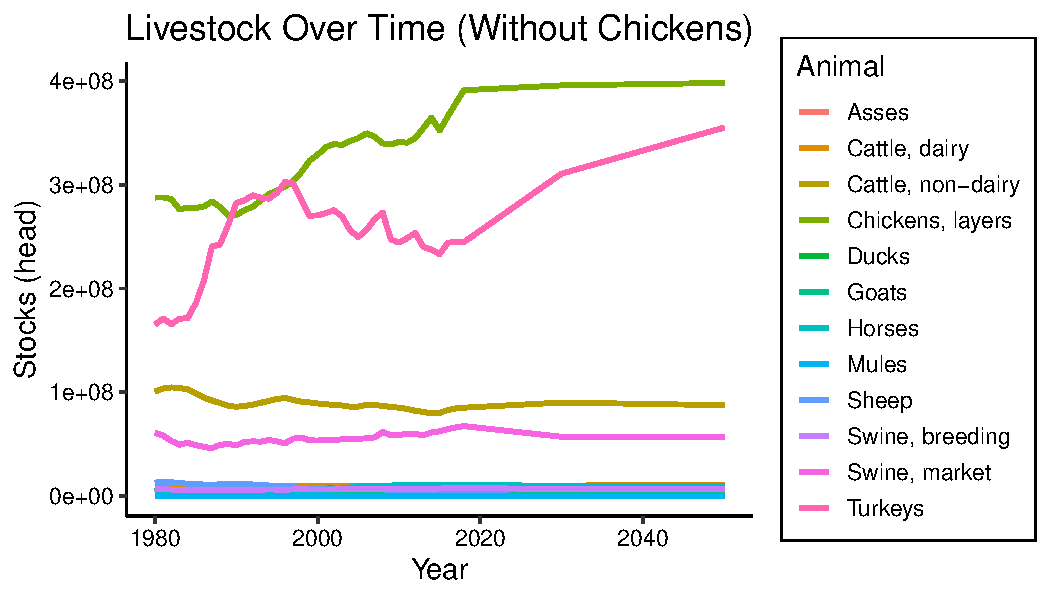
\includegraphics{SultzerSwit_ENV872_Project_files/figure-latex/no.chix-1.pdf}
\caption{Livestock Over Time (Without Chickens)}
\end{figure}

\newpage

\hypertarget{analysis}{%
\section{Analysis}\label{analysis}}

\hypertarget{research-question-1}{%
\subsection{Research Question 1}\label{research-question-1}}

To answer the first research question, the overall methane production
for all livestock was evaluated with a time series analysis. Since
methane was only calculated once a year, there was no seasonality to the
data, and the time series was not able to be decomposed. However, a
Mann-Kendall test was performed, which confirmed that there was a
significant trend (p-value = 0.00011). From data exploration, it can be
seen that overall the trend is increasing: methane emissions between
1980 and 2018 have increased across 13 livestock in the United States
(Figure 1).

From visualizing the total emission rates, dairy cattle and market swine
showed the highest emission rates. A time series analysis was conducted
to determine if there was a significant trend. The Mann-Kendall test
confirmed that a significant trend was present for both animals (p-value
for cattle \textless{} 0.001, p-value for swine \textless{} 0.001).
Dairy cattle (Figure 6) had an overall negative trend in emissions while
market swine had a positive trend (Figure 7).

\begin{figure}
\centering
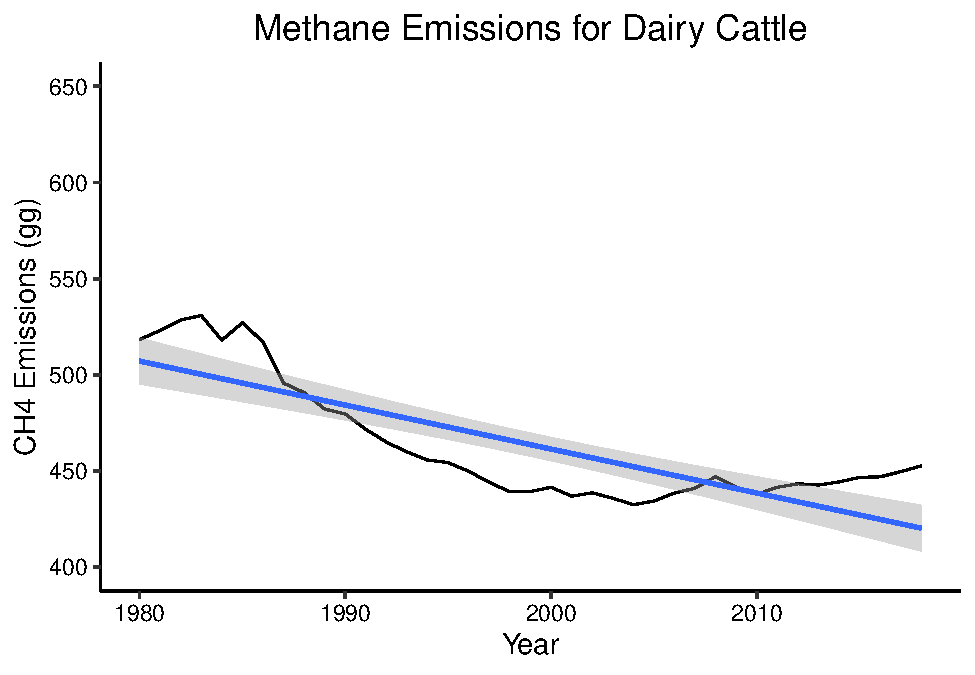
\includegraphics{SultzerSwit_ENV872_Project_files/figure-latex/dairy.cattle.ts-1.pdf}
\caption{Methane Emissions of Dairy Cattle}
\end{figure}

\begin{figure}
\centering
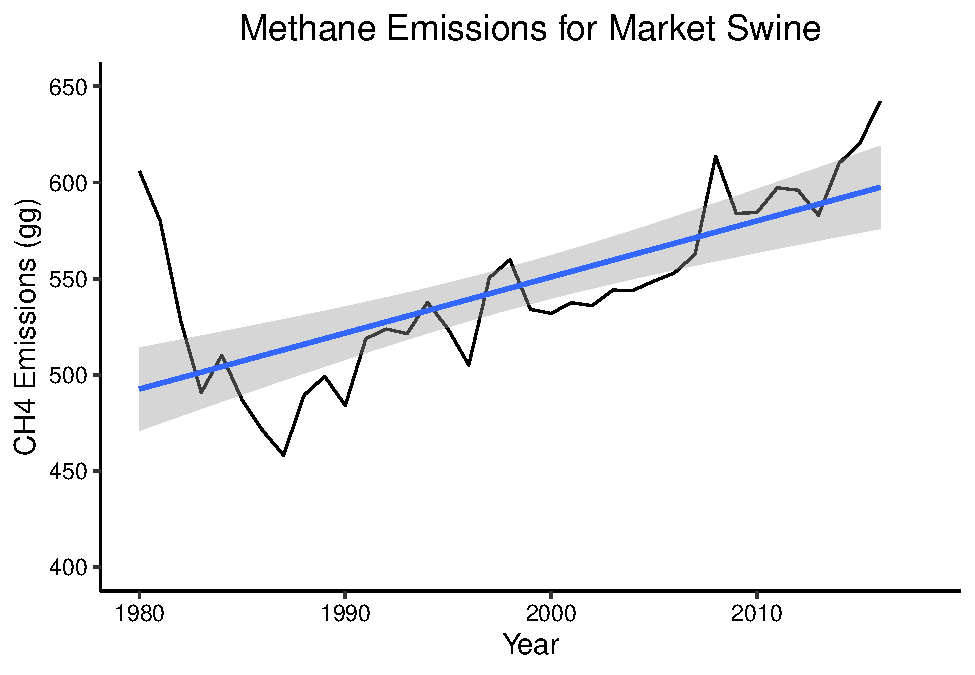
\includegraphics{SultzerSwit_ENV872_Project_files/figure-latex/market.swine.ts-1.pdf}
\caption{Methane Emissions of Market Swine}
\end{figure}

\hypertarget{research-question-2}{%
\subsection{Research Question 2}\label{research-question-2}}

To answer the second research question, a one-way ANOVA test was
conducted to evaluate whether the different animals, on average, have
different emission rates. To begin this process, the emission rates were
checked for normality. The important assumption for generalized linear
models is the normality of residuals. The Shapiro-Wilk test showed that,
of the 13 livestock, only ducks, breeding swine, and market swine were
normally distributed. When viewing a Q-Q plot, once can see the data
does not follow a normal distribution (Figure 8). Lastly, Bartlett's
test for homogeneity of variances was run, which revealed that the
variances were not equal (p \textless{} 0.001). Even though all of the
tests for normality failed, we proceeded on with the analysis.

\begin{figure}
\centering
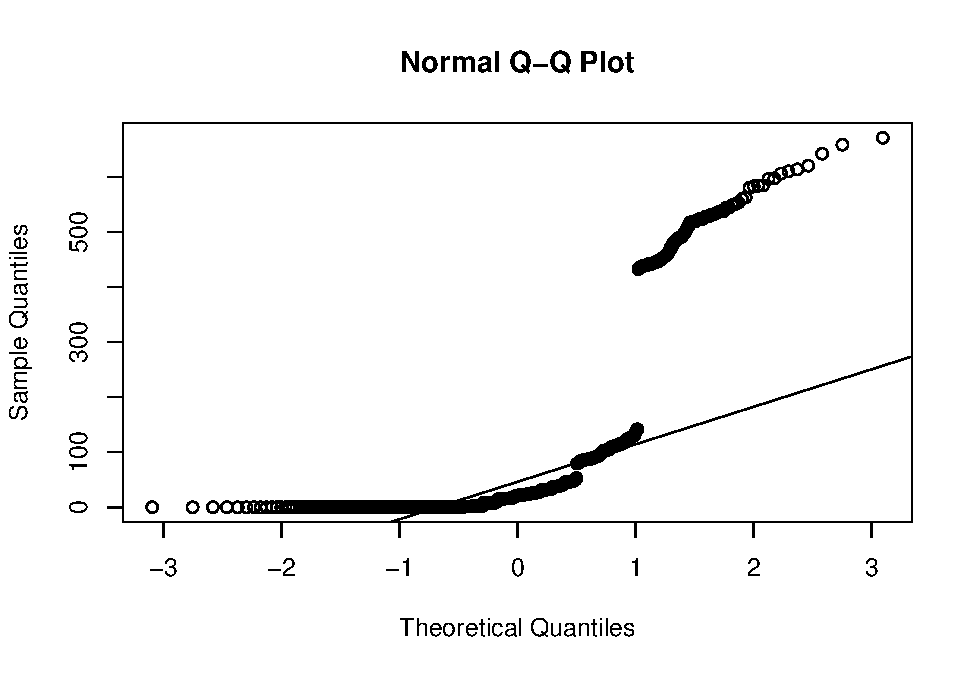
\includegraphics{SultzerSwit_ENV872_Project_files/figure-latex/unnamed-chunk-4-1.pdf}
\caption{QQ plot}
\end{figure}

Analysis then revealed that there was a significant difference in mean
emissions among animals (ANOVA; F: 4394 on 12 and 494
DF,p\textless0.05). But which animals had different means? A Tukey's HSD
test showed which means were different between the animals. Groupings
for pair-wise relationships were extracted, where the letters in Figure
9 represent the different groupings. Thus, asses, ducks, goats, mules,
and sheep all had statistically similar emission rates (Figure 9). Most
of the other animals, such as market swine and dairy cattle, have their
own grouping.

\begin{figure}
\centering
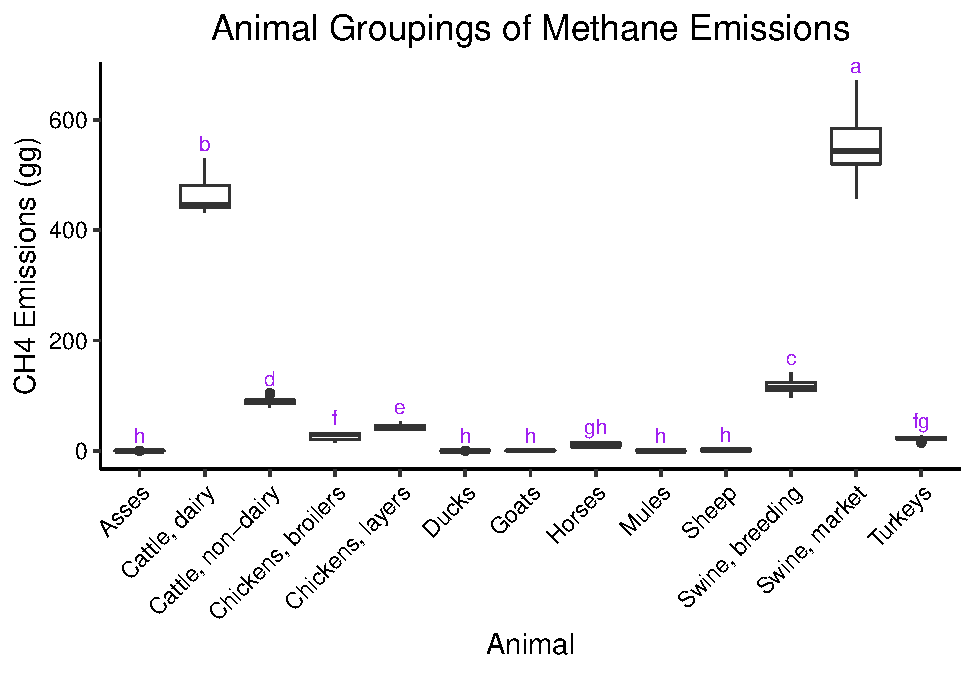
\includegraphics{SultzerSwit_ENV872_Project_files/figure-latex/anova results-1.pdf}
\caption{Animal Groupings of Methane Emissions}
\end{figure}

\newpage

\hypertarget{summary-and-conclusions}{%
\section{Summary and Conclusions}\label{summary-and-conclusions}}

With approximately a tenth of all methane emissions coming from manure
collections ponds, amounts of manure must be considered and properly
managed (Horn, 2018). To summarize, this project investigated how
methane emissions changed over time and how they differed between
livestock. Analysis revealed a significant upward trend in emissions
over time across all selected livestock in the USA. The animals with the
highest emissions, dairy cattle and market swine, exhibited significant
trends with dairy cattle decreasing and market swine increasing from
1980-2018. A one-way ANOVA test confirmed that there were significant
differences in methane emission rates between animals. The Tukey's HSD
test resulted in 8 groups, with asses, ducks, goats, mules, and sheep
being paired in the lowest emitting group. Dairy cattle and market swine
had their own groups and were the highest emitters.

Further analysis could include researching the reasons behind the
decrease in total methane emissions between \textasciitilde1980-1985.
Within this dataset, additional research avenues include assessing
trends in other green house gases, including nitrous oxide and carbon
dioxide emissions. Our research did not include methane emissions from
non-manure sources, such as cattle burping. However, recent strides in
methane reduction research include innovative solutions to limiting
methane produced and emitted by livestock. Such methods include burp
backpacks and vaccinations for reducing methane producing microbes
(Bustamante, 2008).

\newpage

\hypertarget{references}{%
\section{References}\label{references}}

Bustamante, J. (2008, July 8). Cow burps help Argentines study climate
change. Reuters.
\url{https://www.reuters.com/article/us-argentina-cows/cow-burps-help-argentines-study-climate-change-idUSN0830630220080709}.

FAO (2020). FAOSTAT Emissions Database, Agriculture, Manure Management
{[}Data set{]}. \url{http://www.fao.org/faostat/en/\#data/GM}

Horn, P. (2018, October 24). Livestock-based methane emissions
{[}Infographic{]}. Inside Climate News; EPA; FAO.
\url{https://insideclimatenews.org/news/24102018/infographic-farm-soil-carbon-cycle-climate-change-solution-agriculture/}

Watts, G. (2019, August 6). The cows that could help fight climate
change. BBC.
\url{https://www.bbc.com/future/article/20190806-how-vaccines-could-fix-our-problem-with-cow-emissions}

\end{document}
